\documentclass{standalone}
\usepackage{PhysicalChemistryNote}
\begin{document}
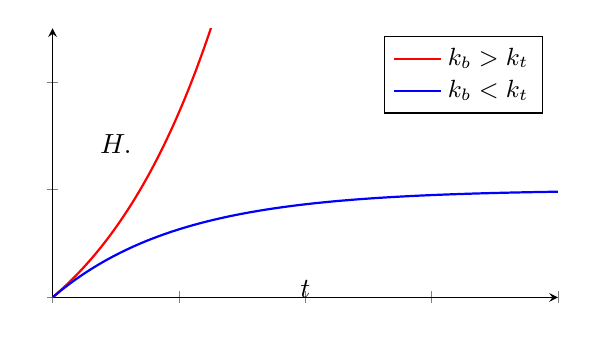
\begin{tikzpicture}
    \begin{axis}[
        width = 8cm,
        height = 5cm,
        legend pos = north east,
        x label style={at={(axis description cs:0.5,0.1)},anchor=north},
        y label style={at={(axis description cs:0.125,0.5)},rotate=270,anchor=south},
        xlabel = {$t$},
        ylabel = {$\con{H.}$},
        axis lines = left,
        ymax = 5,
        domain = 0:8,
        samples = 400,
        xticklabels={},
        yticklabels={}
    ]
    \addplot [thick, red] {2*(e^(0.5*x)-1)};
    \addlegendentry{\small{$k_b>k_t$}}
    \addplot [thick, blue] {-2*(e^(-0.5*x)-1)};
    \addlegendentry{\small{$k_b<k_t$}}
    \end{axis}
\end{tikzpicture}
\end{document}